\documentclass[a4paper, 14pt]{article}%тип документа
\usepackage[14pt]{extsizes}
%отступы
\usepackage[left=2cm,right=2cm,top=2cm,bottom=3cm,bindingoffset=0cm]{geometry}

%Русский язык
\usepackage[T2A]{fontenc} %кодировка
\usepackage[utf8]{inputenc} %кодировка исходного кода
\usepackage[english,russian]{babel} %локализация и переносы

%Вставка картинок
\usepackage{wrapfig}
\usepackage{graphicx}
\graphicspath{{pictures/}}
\DeclareGraphicsExtensions{.pdf,.png,.jpg}

%Графики
\usepackage{multirow}
\usepackage{pgfplots}
\pgfplotsset{compat=1.9}

%Математика
\usepackage{amsmath, amsfonts, amssymb, amsthm, mathtools}

%Заголовок
\author{Валеев Рауф Раушанович \\
группа 825}
\title{\textbf{Вопрос по выбору  \\ 
Исследование взаимной диффузии газов}}
\begin{document}
\maketitle

\section*{Теория}
\subsection*{Общие понятия}
Диффузией называют самопроизвольное проникновение веществ друг в друга, происходящее вследствие хаотичного теплового движения молекул. При перемешивании молекул разного сорта говорят о взаимной (или концентрационной) диффузии.
\subsection*{Законы Фика}
Пусть имеется труба сечением $\Omega$ наполненная раствором какого-либо вещества (рис.1).
\begin{figure}[h]
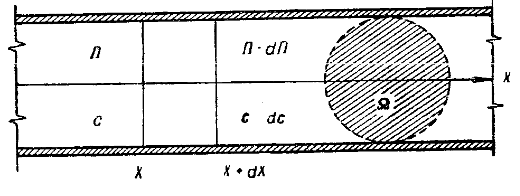
\includegraphics[width = \textwidth]{1.png}
\textbf{\caption{Схема процесса диффузии к выводу законов Фика}}
\end{figure}
Концентрация вещества убывает по направлению оси $x$. Тогда, если мысленно вырезать в этой трубе элементарный слой, заключенный между $x$ и $x + dx$ (толщина которого равна $dx$, а объем $\Omega dx$), то слева от него концентрация и осмотическое давление будут иметь соответственно значения $c$ и $P$, а справа - $c-dc$ и $P-dP$. В результате этого на элементарный слой в направлении оси $x$ будет действовать избыточная сила $\Omega dP$, а на каждую частицу в слое $\Omega dx$, избыточная сила равная
\[-\dfrac{\Omega dP}{cN_a \Omega dx} = -\dfrac{dP}{cN_a dx}\]
Под действием силы осмотического давления частицы должны двигаться по направлению оси $x$ со скоростью $\omega$, определяемой из уравнения
\[w  k = -\dfrac{dP}{c N_a dx}\]
где $k$ - коэффициент внутреннего трения.

Предполагая, что к раствору применимы законы идеальных газов, и представляя 
\[dP = RTdc\]
получаем 
\[\omega k = -\dfrac{RT}{cN_a} \cdot \dfrac{dc}{dx}\]
Отсюда 
\[\omega = -\dfrac{RT}{k} \cdot \dfrac{1}{cN_a} \cdot \dfrac{dc}{dx}\]
за время $dt$ через сечение $\Omega$ пройдет число частиц, равное 
\[dn = \omega \Omega c N_a dt\]
или если исключить $\omega$
\[dn = -\dfrac{RT}{k} \Omega \dfrac{dc}{dx}dt\]
Пусть $\dfrac{RT}{k} = D$ тогда 
\[dn = - D \Omega \dfrac{dc}{dx} dt\]
Или, если выразить через плотность потока, то получим
\[j = \dfrac{dn}{\Omega dt} = -D \dfrac{dc}{dx}\]
Это уравнение обычно называют \textit{\textbf{1 законом Фика}}. Коэффициент $D$ называют коэффициентом диффузии имеющее размерность $[\text{см}^2 c^{-1}]$

При выводе первого закона Фика предполагалось, что градиент концентрации не меняется с течением времени: не зависит от $x$. Первый закон Фика выражает процесс стационарной диффузии. Однако это не всегда так. Так, например, если в левом краю трубки находится твердое тело, способное растворятся в жидкости, наполняющем трубку, то концентрация раствора будет изменятся в пространстве и времени. 

В элементарный слой $dx$ за время $dt$ войдет число частиц, равное 
\[dn = -D \Omega \dfrac{dc}{dx} dt\]
а выйдет за то же время $dt$
\[dn' = -D \Omega \left[ \dfrac{dc}{dx} - \dfrac{d}{dx} \left( \dfrac{dc}{dx} \right) dx \right] dt \]
Отсюда следует что в элементарном слое останется 
\[dn - dn' = D \Omega \left(\dfrac{\partial^2c}{\partial x^2} \right) dx \cdot dt\]
но 
\[\dfrac{dn - dn'}{\Omega dx} = \dfrac{dn - dn'}{dV} = dc\]
и в итоге мы получаем, что 
\[\left( \dfrac{\partial c}{\partial t} \right)_x = D \left(\dfrac{\partial^2c}{\partial x^2} \right)_t\]
Последнее уравнение представляет собой общее дифференциальное уравнение диффузии и является математическим выражением \emph{\textit{\textbf{2 закона Фика}}}.
\subsection*{Конкретно в эксперименте}
Диффузия в системе, состоящей из двух компонентов $a$ и $b$ (бинарная
смесь), подчиняется закону Фика: плотности потока компонентов $j_{a, b}$(количество частиц, пересекающих единичную площадку в единицу времени) пропорциональны градиентам их концентраций $\nabla c_{a,b}$, что в одномерном случае можно записать как
\end{document}
